We measured the time to simulate various formulations of the SIRHD model to highlight the effects of stratification, abstraction, and bounding.  We defined a series of stratification, abstraction, and bounding operations as follows.  Starting with the base model $(\Omega, \Theta)$, we either bound the model $(\Omega^B, \Theta^B)=\text{Bound}(\Omega, \Theta)$, or stratify the model $(\Omega^S, \Theta^S)=\text{Stratify}(\Omega, \Theta)$.  Each stratified model $(\Omega^S, \Theta^S)$ is stratified again differently $(\Omega^{S'}, \Theta^{S'})=\text{Stratify}(\Omega^S, \Theta^S)$, bounded $(\Omega^B, \Theta^B)=\text{Bound}(\Omega^S, \Theta^S)$, or abstracted $(\Omega^A, \Theta^A)=\text{Abstract}(\Omega^A, \Theta^A)$.  Each abstracted model $(\Omega^A, \Theta^A)$ is  bounded $(\Omega^B, \Theta^B)=\text{Bound}((\Omega^A, \Theta^A)$, or abstracted again $(\Omega^{A'}, \Theta^{A'})=\text{Abstract}(\Omega^A, \Theta^A)$.  While it is also possible to stratify an abstracted model, we don't explore this operation here.

Figure \ref{fig:sirhd_experiment_layout} describes how we developed models from the SIRHD base model.  We used several stratifications, and then applied abstractions that reversed the stratifications.  Each abstraction was bounded so that we could simulate the model.  We organized the models in the fashion so that we could demonstrate the time to simulate each model.  In the figure, the models are aligned vertically to indicate which models represent the same level of detail.  For example, the base model and the most-abstract abstraction have the same number of states, transitions, and parameters.  Likewise, reversing the last stratification with the first abstraction results in a model that is the same size as the one prior to the last stratification.  Bounding an abstracted model will increase its size polynomially, whereas stratifying it will increase its size exponentially.  The runtime results tables arrange the models in a similar fashion.  The first column of results increases the model size by stratification from the top to the bottom, and the second column decreases the model size from the top to the bottom.


\begin{figure}
	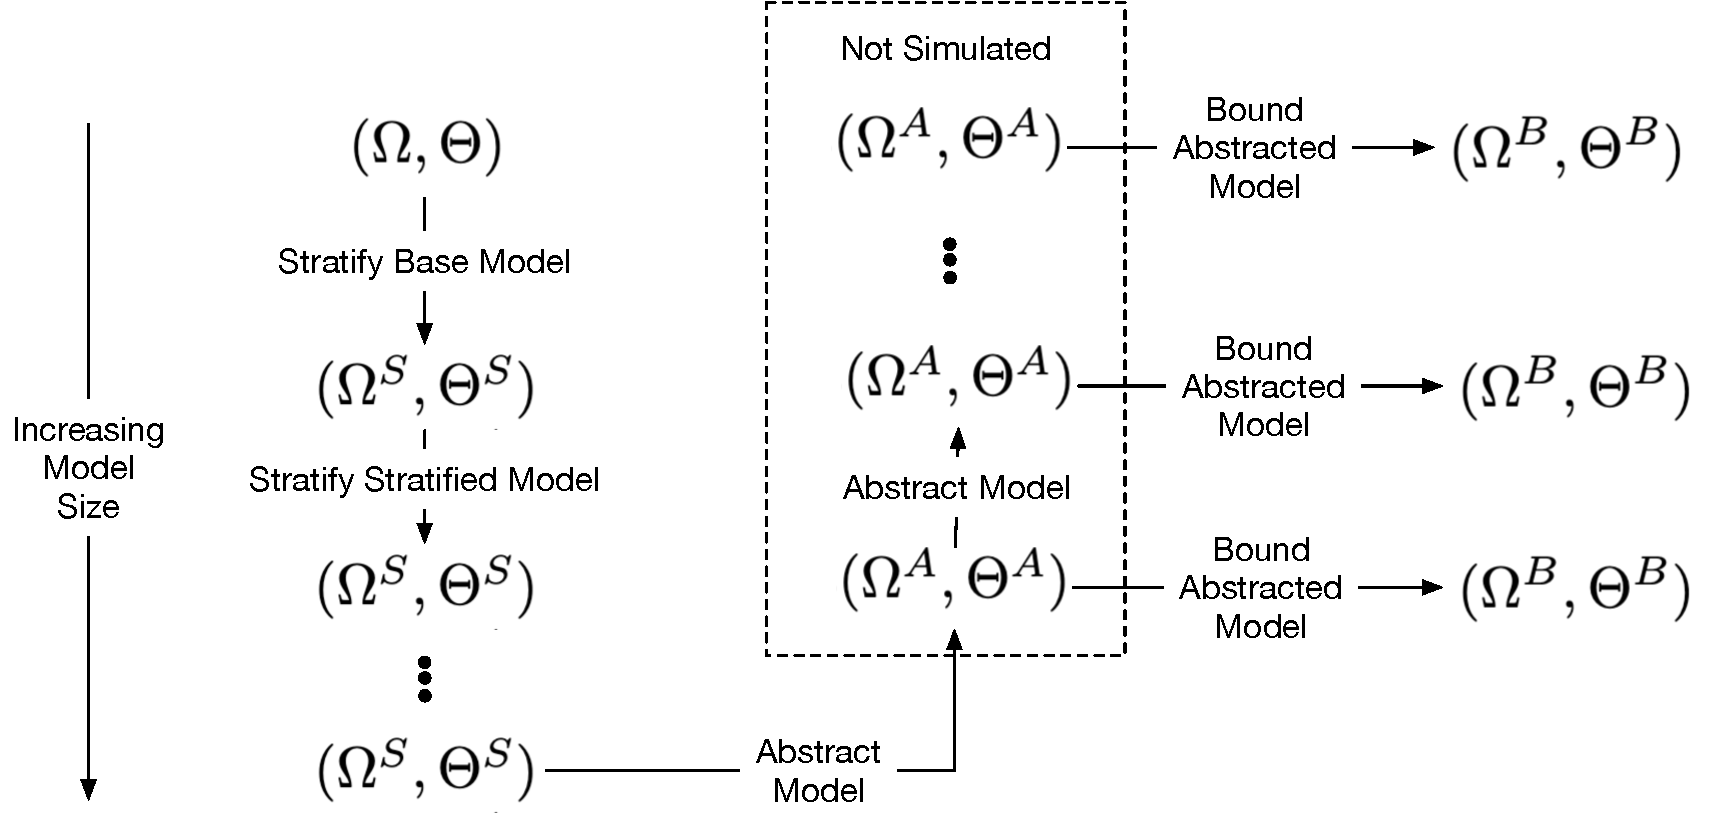
\includegraphics[width=\linewidth]{fig/sirhd_experiment_layout.pdf}
	\caption{\label{fig:sirhd_experiment_layout} Conceptual relationships between model formulations.  The base model can be stratified a number of times.  The final stratified model is abstracted to reverse the stratifications.  Each abstracted model is bounded so that it can be simulated. The dashed box indicates which model are not simulated.}
\end{figure}

\begin{table}\centering
	\begin{tabular}{|r||r|r||r|r|}
		\hline      & \multicolumn{2}{|c||}{3 Age Levels} & \multicolumn{2}{|c|}{5 Age Levels}                              \\
		\hline	Model & Stratified                          & Bounded                            & Stratified   & Bounded     \\
		            &                                     & Abstracted                         &              & Abstracted  \\	\hline
		0           & 0.57                                & 5.26                               & 0.54         & 5.35        \\
		1           & 0.76                                & 7.18                               & 0.69         & 6.93        \\
		2           & 1.33                                & 5.92                               & 2.86         & 7.43        \\
		3           & 2.18                                & {\bf 9.93}                         & 6.29         & {\bf 22.98} \\
		4           & 3.34                                & 9.50                               & 6.17         & 27.63       \\
		5           & 3.88                                & 14.25                              & 11.46        & 52.81       \\
		6           & 5.36                                & 22.84                              & 19.47        & 108.55      \\
		7           & 7.31                                & 23.12                              & 22.97        & 114.84      \\
		8           & 7.13                                & 28.87                              & 26.41        & 143.46      \\
		9           & 8.14                                & 34.59                              & 39.39        & 200.15      \\
		10          & 9.25                                & 32.94                              & 36.55        & 209.17      \\
		11          & 12.36                               & 41.55                              & 49.47        & 245.51      \\
		12          & 12.96                               & 50.17                              & 58.79        & 319.67      \\
		13          & 11.49                               & 56.79                              & 61.23        & 292.44      \\
		14          & 13.73                               & 67.72                              & 66.92        & 361.31      \\
		15          & {\bf 15.17}                         & -                                  & {}\bf 83.80} & -           \\	\hline
	\end{tabular}
	\caption{\label{tab:sirhd_results}  Runtime in seconds to simulate each model formulation.  Model 0 in the Stratified column is the base model.  Models 1-15 in the Stratified column are successive stratifications.  From model 14 to 0 in the Bounded Abstracted column each is a successive abstraction.  The bolded number in the Stratified column is the fully stratified model that we assume is the starting point for analysis.  The bolded number in the Bounded Abstracted column is the smallest model that allows us to confirm the model constraint is satisfied.}

\end{table}

Table \ref{tab:sirhd_results} lists runtime results in seconds to simulate each SIRHD model variation.  Each instance seeks to check a constraint that assesses whether over 200 days the number of infected is no more than 30\% of the population ($N=1.5e9$).  We use 15 stratifications on the model, three for each of the state variables $S$, $I$, $R$, $H$ and $D$.  The three stratifications involve stratifying each state variable into vaccinated and unvaccinated groups (e.g., $S_{vac}$ and $S_{unvac}$), the vaccinated group into age groups (e.g., $S_{vac,0}$, $S_{vac,1}$, $S_{vac,2}$, ...), and the unvaccinated group into age groups (e.g., $S_{unvac,0}$, $S_{unvac,1}$, $S_{unvac,2}$, ...).  We report results for either three or five age groups.  The model index 0-15 refers to successive stratifications of the base model 0 in the Stratified column.  Similarly, the Bounded Abstracted column refers to successive abstractions of the models, where model 14 is the abstraction of model 15 in the Stratified column, and model 13 is the abstraction of model 14 in the Bounded Abstracted column.

We construct the most abstract model 0 from a series of stratifications and abstractions.  It is an over-approximation of the most stratified model that may allow us to prove the constraint is satisfied.  The abstract bounded model represents lower and upper bounds on the number of infected, and if the upper bound is less than 30\% of $N$ (checked through simulation) then we do not need to simulate the most stratified model 15 (our reference model formulation).  The bounded abstract model 0 can be inconclusive if 30\% of $N$ falls between the lower and upper bounds on the number of infected.  By considering successively less abstract models (i.e., proceeding from model 0 to model 1), we expect the lower and upper bounds to tighten.  The bolded time in the Bounded Abstracted model column is the runtime of the first model formulation (starting from model 0) where we can prove that the upper bound on the number of infected is less than 30\% of $N$.  Therefore, if we need to simulate Bounded Abstracted models 0 through 3, we require 28.29  and 42.69 seconds, respectively, for either three or five age groups.  Compared to the time to simulate the largest Stratified model 15, it takes 15.17 or 82.80 seconds respectively.  The savings due to abstraction reduces runtime by one half when there are five age groups, but doubles the runtime when there are three age groups.  This illustrates the trade-off between simulating several abstract models versus one large stratified model.  When the abstract models can capture the important model dynamics using bounds and the number of collapsed stratification levels is large, then abstraction is a win.  